
%------------------------------------------------------------------------------
% 
% Lightning talk on signal transmission
% title:  signal-transmission.tex
% author: Dominik Gedon
% date:   14.12.2020
%
% todo: replace pictures/digrams with self generated ones
%------------------------------------------------------------------------------
\documentclass[handout,ngerman]{beamer}

\usepackage{beamerthemesplit} %// Activate for custom appearance
\usepackage[T1]{fontenc}
\usepackage{inputenc}
\usepackage{graphicx}
\usepackage{svg}
\usepackage{amsmath}
\usepackage[font=small]{caption}
\usepackage{xcolor}
\usepackage{appendixnumberbeamer}
\usepackage{siunitx}
\usepackage{wrapfig}
\usepackage{hyperxmp, hyperref}
\usepackage[
	type={CC},
	modifier={by-sa},
	version={4.0},
	lang={german}
]{doclicense}
\sisetup{
	range-phrase = to,
	per-mode = fraction,
	inter-unit-product = cdot,
	detect-family = false
} 
\usetheme{metropolis}

%------------------------------------------------------------------------------
% definitions 
%------------------------------------------------------------------------------
\newcommand\titlename{Signal\"ubertragung }
\graphicspath{./figures/}
\metroset{sectionpage=simple, subsectionpage=none, numbering=fraction}
\setbeamertemplate{frame footer}{\titlename | Dominik Gedon}


%---------------------------------------------------------------------------------------
%---------------------------------------------------------------------------------------
\title[\titlename]{\titlename}
%\subtitle{Nachrichtentechnische Systeme}
\author{Dominik Gedon}
\date{14. Dezember 2020}

\begin{document}

% title page
\maketitle

% Table of contents
\begin{frame}[plain]{Inhalt}
	\setbeamertemplate{section in toc}[sections numbered]
	\tableofcontents[hideallsubsections]
\end{frame}


%---------------------------------------------------------------------------------------
\section{Grundlagen}
%---------------------------------------------------------------------------------------
\begin{frame}{Grundlagen}
	\textbf{Ziel}
	\begin{itemize}
		\item \"Ubertragung von Informationen \"uber
		\begin{itemize}
			\item den Raum (von Ort zu Ort)
			\item die Zeit (Speicherung)
		\end{itemize}
		\item m\"oglichst effizient
	\end{itemize} 
	
	\textbf{Anwendung}
	\begin{itemize}
		\item Netzwerke (LAN, WLAN,  Mobile Kommunikation)
		\item IT Systeme (Computer, Smartphones, etc.)
		\item Speichermedien (CD, DVD, Blu-ray disk, HDDs)\newline
		$\Longrightarrow$ Fast \textbf{\alert{\"uberall}}	
	\end{itemize} 
\end{frame}


\begin{frame}{Signal\"ubertragung}
	\begin{figure}[htbp]
 	 	\centering 	
 		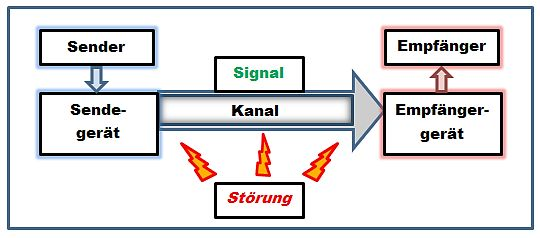
\includegraphics[scale=0.8]{/figures/signal_transmission1} 	 
 		\caption {Sender-Empf\"anger-Modell \cite{sender-empfaenger}}
	\end{figure}
\end{frame}


\begin{frame}{Signale}
	\textbf{Was ist ein Signal?}
	\begin{itemize}
		\item Repr\"asentation einer Information durch einen physikalischen Prozess
		\item z.B.  Spannung \"uber die Zeit, Signaldruck \"uber die Zeit		
	\end{itemize} 
	\textbf{Signalarten}	
	\begin{itemize}
		\item Analoge Signale vs. Digitale Signale
		\item Deterministisch (bekannt) vs. zuf\"allig (unbekannt) 
	\end{itemize} 
\end{frame}

\begin{frame}{Sender}
	\begin{itemize}
		\item Anpassung des Quellensignals an das \"Ubertragungsmedium\newline
		\item Reduzierung der Redundanz + Irrelevanz für die effiziente Nutzung des \"Ubertragungskanals \alert{(Quellenkodierung)}\newline
		\item Redundanzeinfügung zur Sicherung der Nachricht gegen Interferenz und Verfälschung \alert{(Kanalkodierung)}\newline
		\item Effiziente Nutzung der verf\"ugbaren \"Ubertragungsleistung und Signalbandbreite
	\end{itemize} 	
\end{frame}


\begin{frame}{Kanal}
	\textbf{Was ist ein Kanal?}
	\begin{itemize}
		\item Kabel, Luft, Speichermedium
		\item Bestimmt durch die physikalischen Eigenschaften des Übertragungsmediums
	\end{itemize} 
	\textbf{Was passiert?}
	\begin{itemize}
		\item Weiterleitung des übertragenen Signals zum Empfänger
		\item Kanal dämpft das Sendesignal, verursacht Verzerrungen
		\item Unterbrechungen (Rauschen, Interferenzen) überlappen
		\end{itemize} 	
	\end{frame}


\begin{frame}{Empf\"anger}
	\begin{itemize}
	\item Wiederherstellung des Quellsignals aus dem empfangenen Signal\newline
	\item Gewinnung von so viel Information wie möglich über das im empfangenen Signal enthaltene Quellensignal\newline
	\item Anpassung des empfangenen Signals an die Senke
	\end{itemize} 
\end{frame}



%\begin{frame}{Modulation}
%\begin{itemize}[label={-}, itemsep=2ex]	
%	\item Generation of a high-frequency transmission signal
%	
%	\end{itemize} 	
%\end{frame}

\begin{frame}{Kodierung}
\textbf{Was ist Kodierung?}

Eine Abbildungsregel, die jedem Zeichen eines Quellenworts eindeutig eine Zeichenfolge zuordnet.

$ \underbrace{\begin{matrix} (a & b & c)\end{matrix}}
_\text{\textcolor{bleudefrance}{Quellenalphabet}} = \underbrace{\begin{matrix} (0 & 1)\end{matrix}}_\text{\textcolor{mLightBrown}{Zielalphabet}}$\newline\newline\newline
Abbildung: $ \begin{matrix} (a \mapsto 0, b \mapsto 01, c \mapsto 011)\end{matrix}$\newline

\textbf{Beispiel}


$ \underbrace{\begin{matrix} (acabc)\end{matrix}}
_\text{\textcolor{bleudefrance}{Quellenwort}} = \underbrace{\begin{matrix} (0 &011 &0 &01 &011)\end{matrix}}_\text{\textcolor{mLightBrown}{Codewort}}$

\end{frame}


%---------------------------------------------------------------------------------------
\section{Quellenkodierung}
%---------------------------------------------------------------------------------------
\begin{frame}{Wiederholung: Signal\"ubertragung}
	\begin{figure}[htbp]
 	 	\centering 	
 		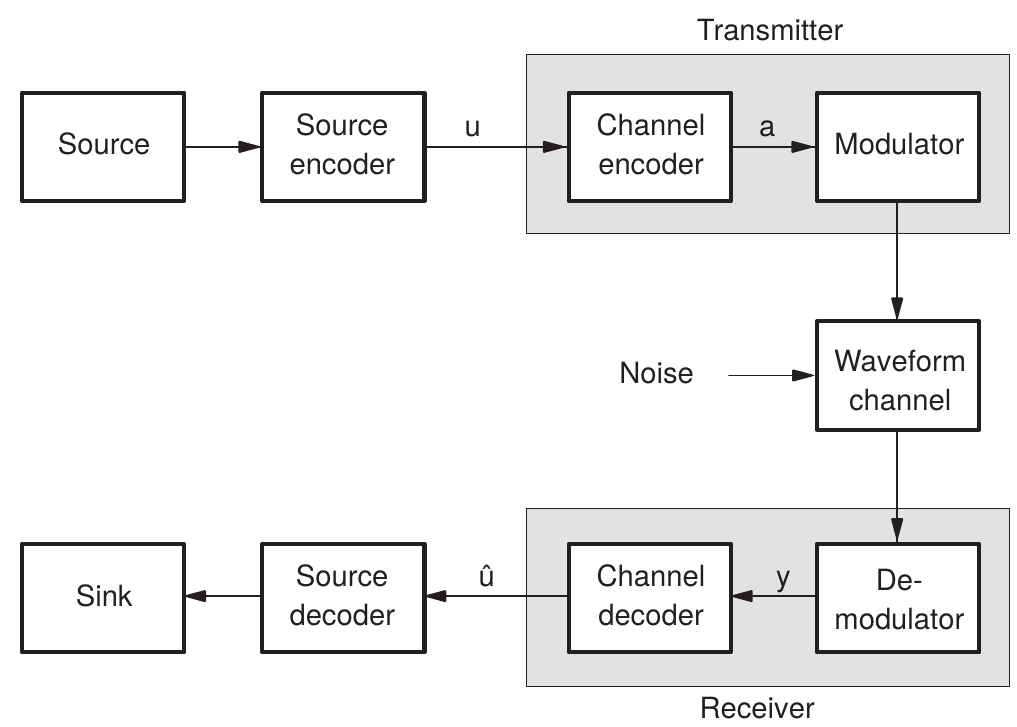
\includegraphics[scale=0.22]{/figures/signal_transmission} 	 
 		\caption {\"Uberblick Signal\"ubertragung \cite{friedrichs}}
	\end{figure}
\end{frame}

\begin{frame}{Quellenkodierung}
	\textbf{Was ist das?}
	\begin{itemize}
		\item Entfernung redundanter Informationen
		\item Kompression von Daten
	\end{itemize} 
	\textbf{Wie wird das erreicht?}
	\begin{itemize}
		\item Abbildung von Quellwörtern mit hoher Wahrscheinlichkeit auf kurze Codewörter
	\end{itemize} 
\end{frame}


\begin{frame}{Quellenkodierung: Beispiel - Huffman Kodierung}
\textbf{Annahme:}\newline
$Pr\{A\} = \textcolor{mLightBrown}{0,8} \newline Pr\{B\} = \textcolor{bleudefrance}{0,2} $
	\begin{figure}[htbp]
 	 	\centering 	
 		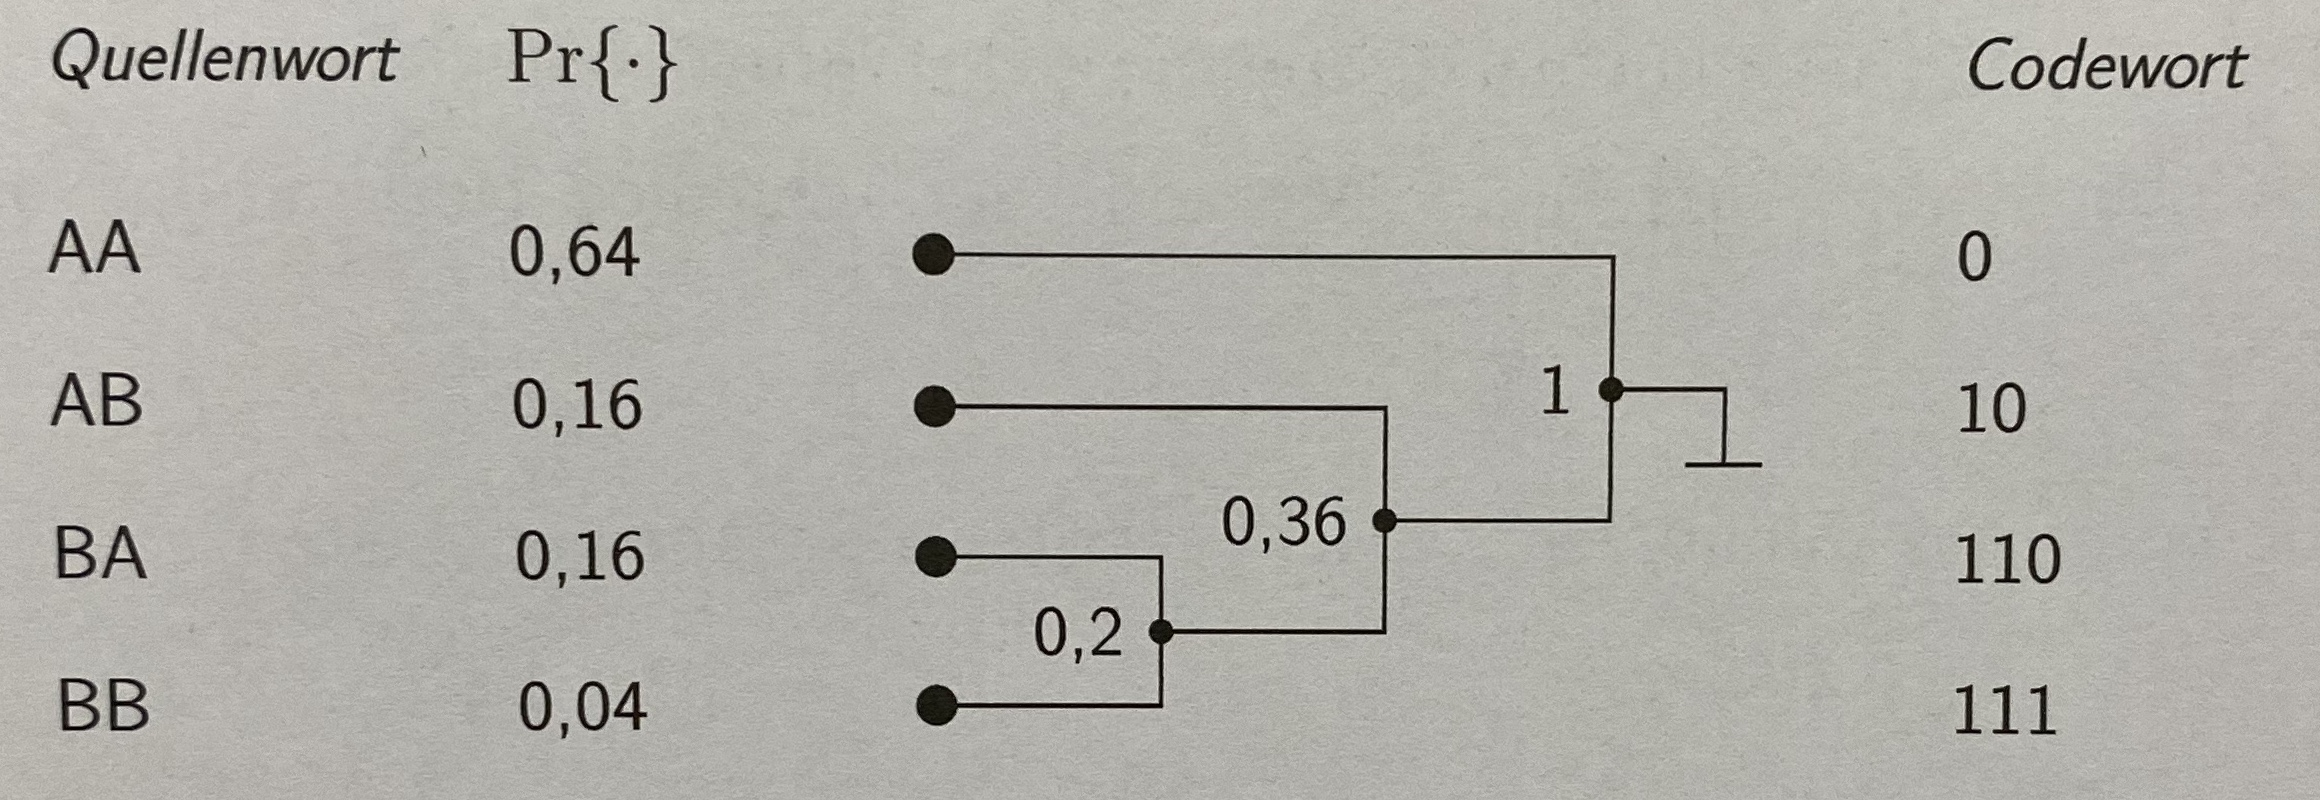
\includegraphics[scale=0.135]{/figures/huffman1} 	 
 		\caption {Beispiel I- Huffman Kodierung \cite{huber}}
	\end{figure}
\end{frame}
%
%\begin{frame}{Quellenkodierung: Beispiel II - Huffman Kodierung}
%	\begin{figure}[htbp]
% 	 	\centering 	
% 		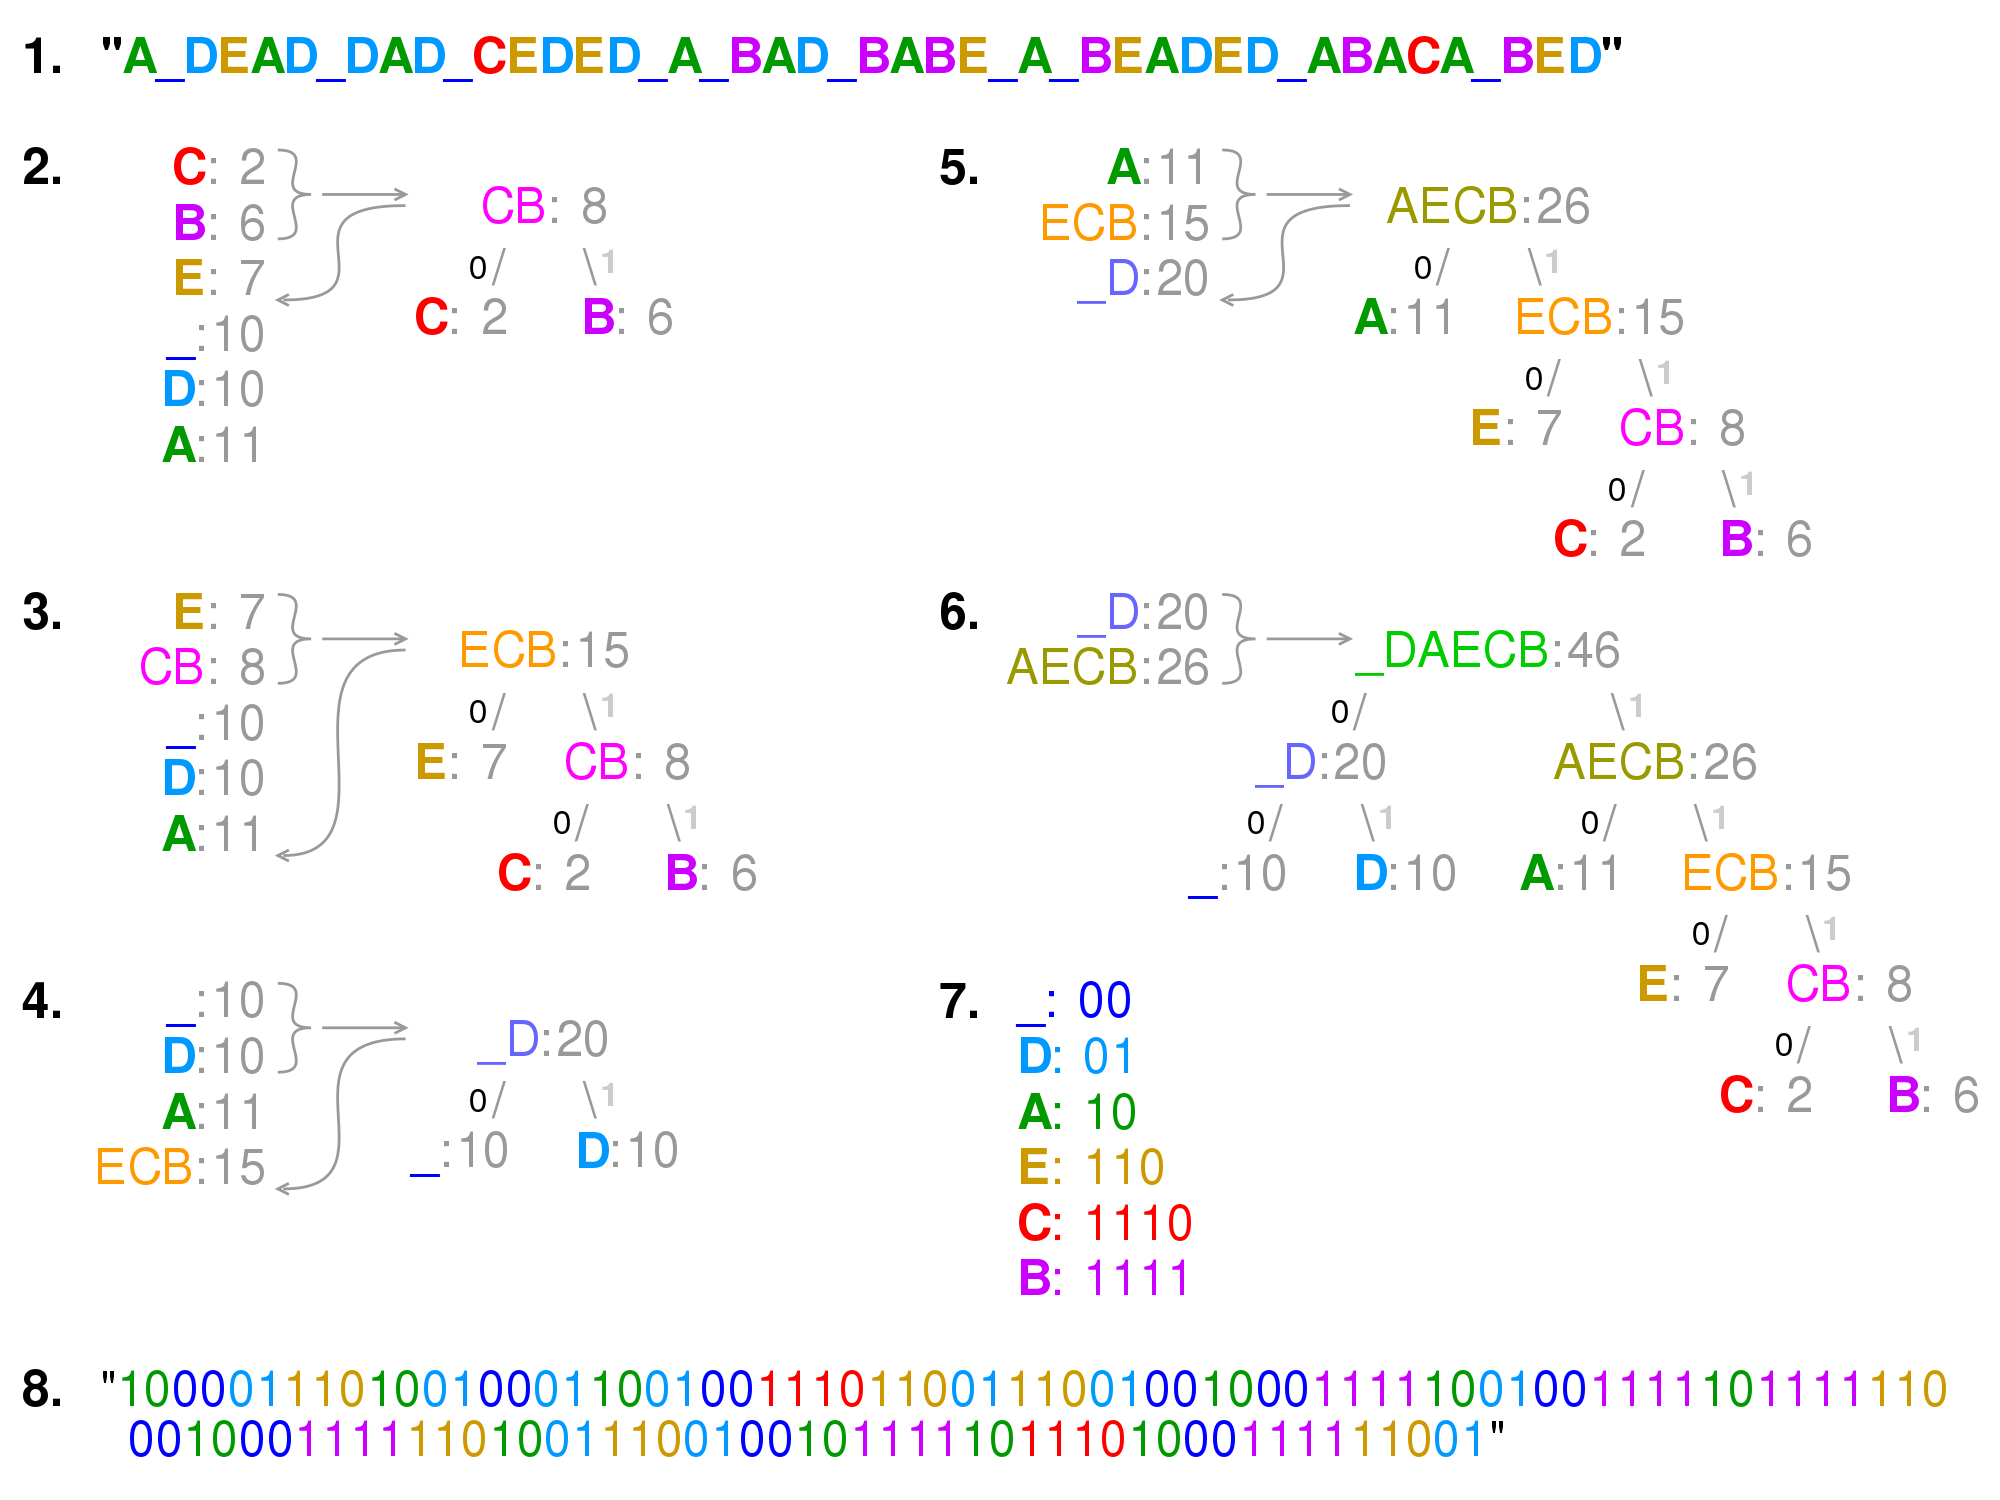
\includegraphics[scale=0.125]{/figures/huffman2} 	 
% 		\caption {Beispiel II - Huffman Kodierung\cite{huffman}}
%	\end{figure}
%\end{frame}


%---------------------------------------------------------------------------------------
\section{Kanalkodierung}
%---------------------------------------------------------------------------------------
\begin{frame}{Wiederholung: Signal\"ubertragung}
	\begin{figure}[htbp]
 	 	\centering 	
 		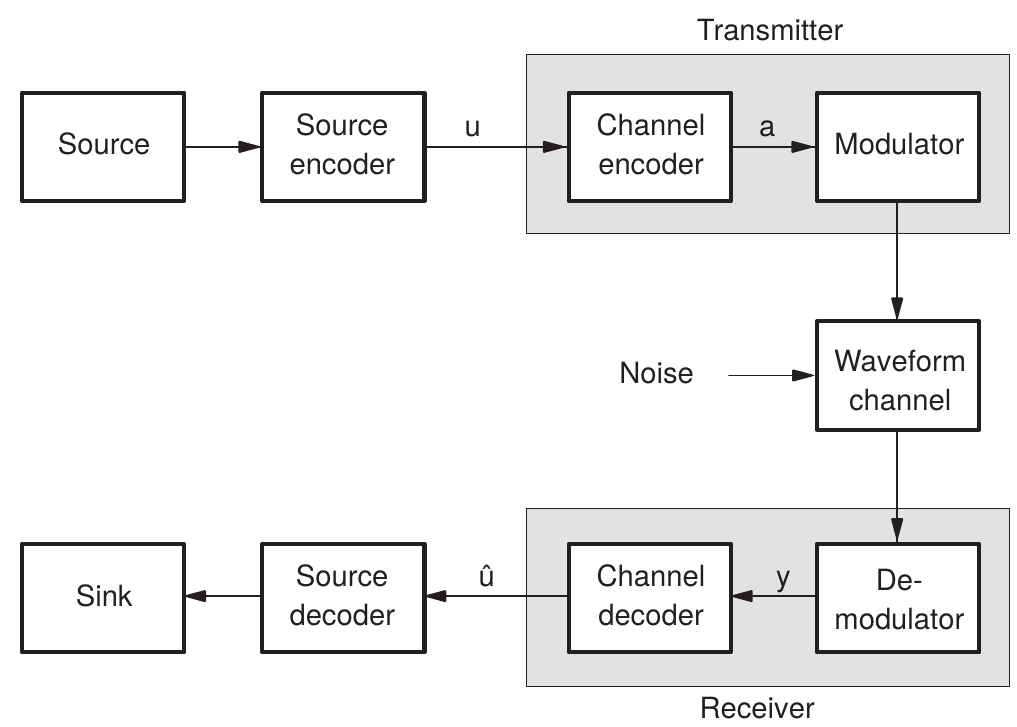
\includegraphics[scale=0.22]{/figures/signal_transmission} 	 
 		\caption {\"Uberblick Signal\"ubertragung \cite{friedrichs}}
	\end{figure}
\end{frame}

\begin{frame}{Kanalkodierung: Was ist das?}
	\begin{itemize}
		\item Bei der Übertragung und Speicherung von Daten muss mit \alert{Fehlern} gerechnet werden
		\item Sichern der Nachricht gegen Fehler \newline
		 $\Longrightarrow$ Hinzuf\"ugen von \textbf{\alert{Redundanz}} auf der Senderseite
		\item Der Empfänger nutzt diese Redundanz, um Fehler zu erkennen und zu korrigieren\newline\newline
	 \textbf{Aufgabe}
		\item \alert{Fehlererkennung} und falls notwendig \alert{Fehlerbeseitigung} basierend auf Redundanz
	\end{itemize}	  
\end{frame}


\begin{frame}{Kanalkodierung: Beispiel}
	\begin{itemize}
		\item International Standard Book Number (\textbf{ISBN})
		\begin{figure}[htbp]
 	 		\centering 	
 			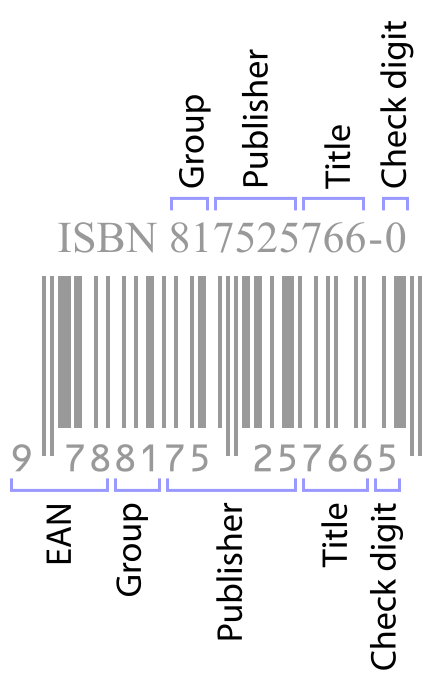
\includegraphics[scale=0.25]{/figures/ISBN} 	 
 			\caption {Eine 10-stellige ISBN und die die zugeh\"orige EAN‑13 \cite{isbn}}
		\end{figure}
	\end{itemize}
\end{frame}

%---------------------------------------------------------------------------------------
\section{Zusammenfassung}
%---------------------------------------------------------------------------------------
\begin{frame}{Zusammenfassung}
	\begin{itemize}
		\item Signalübertragung ist fast überall\newline
		$\Rightarrow$ Die Verarbeitung des Signals ist notwendig\newline
		\item Datenkompression (Quellenkodierung)	\newline
		\item Sichern der Nachricht gegen Fehler (Kanalkodierung)\newline
		 $\Rightarrow$ \textbf{Redundanz}
	\end{itemize}  
\end{frame}


%---------------------------------------------------------------------------------------
\begin{frame}{Quellen}
%---------------------------------------------------------------------------------------
  Get the \LaTeX\ source of this presentation from
  \begin{center}\url{https://github.com/nodeg/presentations}\end{center}
  The presentation \emph{itself} is licensed under a  \href{https://creativecommons.org/licenses/by-sa/4.0/}{Attribution-ShareAlike 4.0 International (CC BY-SA 4.0) License}.
  \begin{center}\doclicenseImage\end{center}
\end{frame}


%---------------------------------------------------------------------------------------
\begin{frame}[allowframebreaks]{Quellen}
%---------------------------------------------------------------------------------------
  \bibliography{signal-transmission}
  \bibliographystyle{abbrv}
\end{frame}


\end{document}
